\documentclass {beamer}

\usetheme {JuanLesPins}
\setbeamertemplate {footline} [frame number]

\usepackage[utf8]{inputenc}
\usepackage[english]{babel}
% \usepackage[ngerman]{babel}

\usepackage{amsmath}
\usepackage{amssymb}
\usepackage{amsfonts}
\usepackage{xcolor}
\usepackage{graphicx}
\usepackage{float}
\usepackage{enumerate}
\usepackage{verbatim}
\usepackage{stmaryrd}

\usepackage{listings}
\lstset{language=C++}

\usepackage{tikz}
\usetikzlibrary{backgrounds}
\usetikzlibrary{arrows,decorations.pathmorphing,positioning,fit,trees,shapes}

\lstdefinestyle{customc}{
  belowcaptionskip=1\baselineskip,
  breaklines=true,
  xleftmargin=\parindent,
  language=C,
  showstringspaces=false,
  basicstyle=\footnotesize\ttfamily,
  keywordstyle=\bfseries\color{green!40!black},
  commentstyle=\itshape\color{purple!40!black},
  identifierstyle=\color{blue},
  stringstyle=\color{orange},
}

\lstdefinestyle{customasm}{
  belowcaptionskip=1\baselineskip,
  frame=L,
  xleftmargin=\parindent,
  language=[x86masm]Assembler,
  basicstyle=\footnotesize\ttfamily,
  commentstyle=\itshape\color{purple!40!black},
}

\lstset{escapechar=@,style=customc}

\title{Monotonic Abstraction for Programs with Muliply-Linked Structures}
\date{WS 2016}
\author{Timotheus Jochum \\ Supervision: David Korzeniewski}

\institute [RWTH-Aachen] {Rheinisch-Westfaelische Technische Hochschule Aachen - Bc. Informatik}
\date{14. Februar 2017}
\subject {Monotonic Abstraction for Programs with Muliply-Linked Structures}

\begin{document}

\begin{frame}[fragile]{}
        \titlepage
\end{frame}

%!TEX root = ./main.tex
\begin{frame}[fragile]{Introduction}
	\pause
	\begin{itemize}
		\item <2-> Verification of programs
		\item <3-> Programs written in a subset of C
		\item <4-> Operating on multiply linked data structures
	\end{itemize}
\end{frame}
%!TEX root = ./main.tex
\begin{frame}[fragile]{Outline}
    \begin{itemize}
        \pause
        \item <2-> Introduction
        \item <3-> Structures
        \item <4-> Heap
        \item <5-> Signatures
        \item <6-> Monotonic Abstraction
        \item <7-> Computing Predecessors
        \item <8-> Reachability Algorithm
        \item <9-> Conclusion
    \end{itemize}
\end{frame}
%!TEX root = ./main.tex
\begin{frame}[fragile]{Structures}
    \begin{itemize}
        \pause
        \item <2-> C structs with two selectors
        \pause
    \end{itemize}
    
    \begin{lstlisting}[style=customc]
        struct A {
            A *next;
            A *prev;
            Data data;
        }    
    \end{lstlisting}

    \begin{itemize}
        \pause
        \item <4-> Allows complex structs
        \pause
    \end{itemize}

    \begin{lstlisting}[style=customc]
        struct B {
            T1 t1;
            T2 t2;
            T3 t3;
            T4 t4;
        }    
    \end{lstlisting}

\end{frame}


%!TEX root = ./main.tex
\begin{frame}[fragile]{Heap}
    
    \pause
    \begin{itemize}
        \item <2-> Vertex and edge labeled graph 
        \item <3-> Each node represents a memory cell
        \item <4-> Each edge represents a pointer/selector
        \item <5-> '\#' represents the \textit{null node}
        \item <6-> '*' represents the \textit{dangling node}
        \item <7-> Labels on nodes for variables
    \end{itemize}

\end{frame}

\begin{frame}[fragile]{Heap}
    
    \pause
    \begin{definition}
        A \textit{heap} is defined as a tuple $(\overline{M}, E, s, t, \tau, \lambda)$
        where:
        \begin{itemize}
            \item <3-> $\overline{M} = M \cup \{\#, *\}$, where $M$ is the set of memory cells
            \item <4-> $E$ is the set of edges
            \item <5-> $s : E \rightarrow M$ is the \textit{source function} 
            \item <6-> $t : E \rightarrow \overline{M}$ is the \textit{target function}
            \item <7-> $\tau : E \rightarrow C$ is the \textit{type function}, where $C = \{1, 2\}$ is the set of selectors
            \item <8-> $\lambda : X \rightarrow \overline{M}$ is the \textit{variable function}, where $X$ is a set of variables
        \end{itemize}
    \end{definition}
\end{frame}

\begin{frame}[fragile]{Heap}
    
    \pause
    Example of a heap:
    \pause
    
    \begin{figure}
        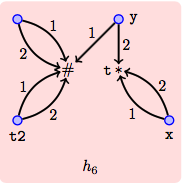
\includegraphics[scale=0.57]{images/Heap6Example.png}
        \\ \tiny{Example Heap \cite{abdulla2013monotonic}}
    \end{figure}

    \pause

    \begin{itemize}
        \item The heap invariant: 
        \item <5-> $\forall c \in C$ $\forall m \in M : |s^{-1}(m) \cap \tau^{-1}(c)| = 1$ \\
    \end{itemize}
\end{frame}

\begin{frame}[fragile]{Heap Transition System}
    
    \pause

    \begin{itemize}
        \item <2-> Subset of C includes the following operations: 
            \begin{itemize}
                \item <3-> Conditions: $x == y$, $x$ !$= y$
                \item <4-> Assignments: $x = y$, $x = y.next(i)$, $x.next(i) = y$
                \item <5-> Allocation: $x = malloc()$ and $free(x)$
            \end{itemize}
        \item <6-> The Transition System is defined as $T = (S, \rightarrow)$
            \begin{itemize}
                \item <7-> $S$ is a set of states which are pairs of $(pc, h)$ where $pc$ is the Program Counter
                \item <8-> $\rightarrow$ reflects the heap manipulation
            \end{itemize}
        \item <9-> Given states $s, s'$, $s \rightarrow s'$ exists if an operation is defined which transforms $h$ into $h'$ 
    \end{itemize}


\end{frame}


%!TEX root = ./main.tex
\begin{frame}[fragile]{Signatures}
    
    \begin{itemize}
        \item <2-> Defined in the same way as heaps except for:
        \item <3-> The \textit{type function} and the \textit{variable function} can be partial
        \item <4-> Less strict invariants: \\
            \begin{itemize}
                \item <5-> $\forall c \in C$ $\forall m \in M : |s^{-1}(m) \cap \tau^{-1}(c)| \le 1$
                \item <6-> $\forall m \in M : |s^{-1}(m)| \le 2$
            \end{itemize}
        \item <7-> Signatures are partial heaps
        \item <8-> What does a Signature actually represent?
    \end{itemize}

\end{frame}

\begin{frame}[fragile]{Signatures}
    
    \pause

    \begin{itemize}
        \item <2-> Signatures represent infinite sets of heaps
        \item <3-> Or in other words:
    \end{itemize}

    \pause 

    \pause

    \medskip

     A signature is a heap with some parts 'missing'. It represents the set of all heaps that have at least the property or structural information described by this signature.
\end{frame}

\begin{frame}[fragile]{Ordering on Signatures}
    
    \pause

    Ordering Steps:

    \pause

    \begin{itemize}
        \item <3-> Isolated cell deletion
        \item <4-> Edge deletion
        \item <5-> Contraction
        \item <6-> Edge decoloring
        \item <7-> Label deletion
    \end{itemize}

\end{frame}

\begin{frame}[fragile]{The Ordering Relation}
    
    \pause

    \begin{definition}
        We say a signature $sig_1$ is smaller than a signature $sig_2$, if there is a sequence of 
        ordering steps that leads from $sig_2$ to $sig_1$, written as $sig_1$ $\sqsubseteq$ $sig_2$.
    \end{definition}

    \pause

    \begin{itemize}
        \item <3-> We say that a heap $h$ satisfies $sig_1$, written as $h \in \llbracket sig_1 \rrbracket$, if $sig_1 \sqsubseteq h$
    \end{itemize}

\end{frame}

\begin{frame}[fragile]{Bad Configurations}
    
    \pause

    \begin{itemize}
        \item <2-> Heap Configurations that should \textbf{never} occur
        \item <3-> Represented as signatures
        \item <4-> Example of a Bad Configuration:
    \end{itemize} 

    \pause 

    \pause

    \pause

    \medskip
    \medskip

    \medskip

    Non-Cyclicity: This bad configuration refers to all structures which have a selector pointing to the same memory cell $m$.

    \pause

    \begin{center}
        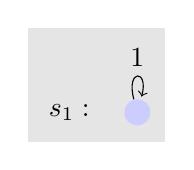
\begin{tikzpicture}
            [scale=.8,auto=left,main node/.style={circle,fill=blue!20}, background rectangle/.style={fill=gray!20}, show background rectangle]
            \node[main node] (1) {};
            \node[text width=1cm, anchor=ost, left] at (0,0) {$s_1:$};
            \path (1) edge [loop above] node {1} (1);
            \end{tikzpicture}
            \qquad
            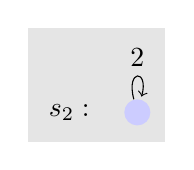
\begin{tikzpicture}
            [scale=.8,auto=right,main node/.style={circle,fill=blue!20}, background rectangle/.style={fill=gray!20}, show background rectangle]
            \node[main node] (1) {};
            \node[text width=1cm, anchor=ost, left] at (0,0) {$s_2:$};

            \path (1) edge [loop above] node {2} (1);
        \end{tikzpicture}
    \end{center}
\end{frame}

%!TEX root = ./main.tex
\begin{frame}[fragile]{Monotonic Abstraction}
    
    \pause

    \begin{definition}

        A transition system T is monotonic if the following holds. For any states $sig_1, sig_2$ and $sig_3$ such that
        $sig_1 \sqsubseteq sig_2$ and $sig_1 \longrightarrow sig_3$, we can always find a state $sig_4$ such that $sig_2 \longrightarrow sig_4$
        and $sig_3 \sqsubseteq sig_4$.
    \end{definition}

    \begin{itemize}
        \item <3-> Our Transition System is not monotonic
        \item <4-> Construct an over approximation
        \item <5-> If the over approximation is valid, the original will also be valid
    \end{itemize}

    \pause
    \pause
    \pause
    \pause

    \begin{definition}

        We say $s \longrightarrow_A s'$ for two signatures $s$ and $s'$ iff there is an $s"$ such that $s" \sqsubseteq s$ and
        $s \longrightarrow s'$. 
    \end{definition}

\end{frame}
%!TEX root = ./main.tex
\begin{frame}[fragile]{Calculating Predecessors}
    
    \pause

    The predecessor function $pre(op)(sig)$:

    \pause

    \begin{itemize}
        \item <3-> Calculates the set of signatures which leads to $sig$ if $op$ is applied
        \item <4-> Definition needed for each operation $op$:
            \begin{itemize}
                \item <5-> $pre($x = malloc()$)(sig)$
                \item <6-> $pre($free(x)$)(sig)$
                \item <7-> $pre($x == y$)(sig)$
                \item <8-> $pre($x != y$)(sig)$
                \item <9-> $pre($x = y.next(i)$)(sig)$
                \item <10-> $pre($x.next(i) = y$)(sig)$
                \item <11-> $pre($x = y$)(sig)$
            \end{itemize}
    \end{itemize}

\end{frame}
%!TEX root = ./main.tex
\begin{frame}[fragile]{Reachability Algorithm}
    
    \pause

    \begin{itemize}
        \item <2-> Backwards Analysis from set of bad configurations $S_{bad}$
        \item <3-> Compute predecessors for every $s \in S_{bad}$
        \item <4-> If a predecessor $p$ is computed with $s' \sqsubseteq p$, where $s'$ is a previously calculated signature, discard $p$
        \item <5-> Repeat until all new computed predecessors are being discarded
        \item <6-> If the set of signatures is disjoint from the initial set of states\\
         $\Rightarrow$ program execution is safe
    \end{itemize}

\end{frame}
%!TEX root = ./main.tex
\begin{frame}[fragile]{Conclusion}
    
    \pause

    \begin{itemize}
        \item <2-> Approach has been implemented in a Java prototype
    \end{itemize}

    \pause

    \begin{figure}
        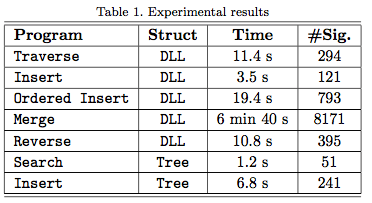
\includegraphics[scale=0.5]{images/ResultTable.png}
        \\ \tiny{Prototype Results \cite{abdulla2013monotonic}}
    \end{figure}
\end{frame}

\begin{frame}[fragile]{Conclusion}
    
    \pause

    \begin{itemize}
        \item <2-> Relatively simple method
        \item <3-> Very generic approach
        \item <4-> Successfully implemented
    \end{itemize}

\end{frame}

\begin{frame}[fragile]{Conclusion}
    
    Any questions?

\end{frame}

\begin{frame}[fragile]{}
    \bibliographystyle{amsalpha}  
    \bibliography{literature.bib}
\end{frame}

\end{document}
